\documentclass[conference]{IEEEtran}

\usepackage{amsmath}
\usepackage{graphicx}
\usepackage{booktabs}
\usepackage{url}
\usepackage[hidelinks]{hyperref}
\usepackage{tikz}
\usepackage{pgfplots}
\pgfplotsset{compat=1.17}
\usetikzlibrary{arrows.meta,positioning}

\begin{document}

\title{A Comparative Planning-and-Control Stack for\\ Autonomous Racing in the CARLA Simulator}

\author{%
\IEEEauthorblockN{Vaibhav Raheja}
\IEEEauthorblockA{\textit{vaibhavvraheja@gmail.com}}
\and
\IEEEauthorblockN{Darian Irani}
\and
\IEEEauthorblockN{Mahi Ranka}
}

\maketitle

\begin{abstract}
Autonomous racing packs the central challenges of self-driving---planning
under kinematic constraints, obstacle avoidance, and trajectory tracking near
the limits of vehicle dynamics---into a single, tightly time-boxed control
loop. This paper reports the design and evaluation of a planning-and-control
stack for an autonomous race car in the CARLA simulator, built against the
GRAIC~2023 (Generalized Racing Intelligence Competition) framework. Rather than
committing to a single paradigm, we implemented and compared a broad set of
methods side by side: search-based global planners (A*, Hybrid~A*, and a
dynamic-programming cost-to-go heuristic), sampling-based planners (RRT and
RRT*), a smooth spline reference generator, a reactive local planner (the
Dynamic Window Approach), and five trajectory-tracking controllers
(proportional--derivative, Stanley, Stanley with an added PID speed loop, LQR,
and MPC). An integrated final agent combines a spline-smoothed reference with a
lookahead proportional steering law and heading-aware speed modulation, and is
the configuration used for scored evaluation. We report scores on five
competition tracks against the naive reference controller shipped with the
framework, analyze the per-track collision logs the harness produces, and
identify where the stack improves on the baseline and where it does not. The
stack beats the baseline on four of the five tracks; the single regression is
localized to one track and is traced to run-off-track terrain collisions rather
than a systemic failure.
\end{abstract}

\begin{IEEEkeywords}
autonomous racing, motion planning, trajectory tracking, CARLA, model
predictive control, path planning
\end{IEEEkeywords}

\section{Introduction}

Autonomous racing compresses the core problems of self-driving into an
unusually demanding setting. A racing agent must perceive nearby obstacles,
plan a feasible path that respects the vehicle's kinematics, and track that
path accurately while operating close to the friction and actuation limits of
the car---and it must do all of this within a fixed per-step time budget. Small
errors in either planning or control compound quickly at speed, so the setting
is a useful stress test for the interaction between the two.

The GRAIC~2023 framework provides a standardized, CARLA-based harness for this
problem. A scenario runner spawns an ego vehicle on one of several fixed
tracks, optionally injects dynamic traffic and pedestrians, and calls a single
fixed agent interface once per simulation tick. At each tick the agent receives
the set of nearby obstacles, a horizon of upcoming track waypoints, the ego
vehicle's current velocity and pose, and the left/right track boundary, and
must return a throttle--steer--brake command within a bounded time. This narrow,
well-defined interface makes the framework a convenient common ground for
comparing planning and control methods on equal terms.

The goal of this project was deliberately breadth-first: rather than tuning one
method in isolation, we explored the design space by implementing multiple
planners and multiple controllers against the same interface, then integrating
the most effective combination into a final agent used for scored runs. This
paper documents that stack, the reasoning behind each component, and the
results obtained on the competition tracks. Our contributions are (i) a single
codebase implementing and exposing more than a dozen planner and controller
variants behind one interface; (ii) an integrated agent that outperforms the
framework's reference controller on four of five tracks; and (iii) an honest
per-track analysis, grounded in the harness's own score and collision logs, of
where the approach works and where it breaks down. A short demonstration is
available online.\footnote{\url{https://youtu.be/n1QGdyXPFZI}}

\section{System Overview}

Every agent variant in the codebase implements the same interface required by
the harness: a per-tick call that is handed the filtered obstacle list, the
upcoming waypoints, the current velocity and transform, and the track boundary,
and that returns a CARLA vehicle-control command. This uniformity is what makes
the planners and controllers interchangeable, and it is the reason the same
scoring harness can be pointed at any variant without modification.

Conceptually, each agent follows the pipeline shown in
Fig.~\ref{fig:pipeline}. The harness supplies the current state and a local
view of the track ahead; a planning stage produces a reference path from the
waypoints while treating nearby obstacles and the boundary as constraints; a
control stage converts the reference and the current state into a steering
angle and a longitudinal (throttle/brake) command; and the harness applies that
command, advances the simulation, and logs any collisions before calling the
agent again. The final agent uses a spline-smoothed reference and a lightweight
lookahead controller, but every stage of the pipeline can be swapped for one of
the alternatives described below.

\begin{figure}[t]
\centering
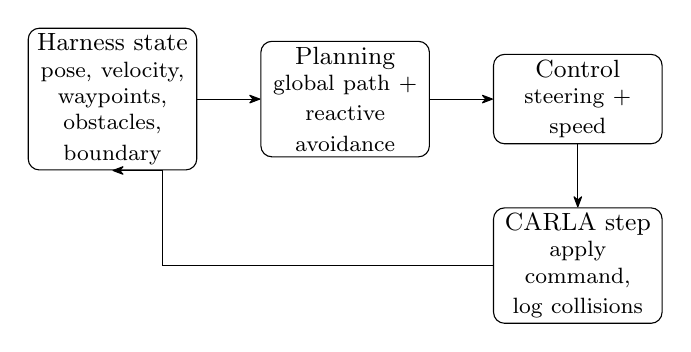
\begin{tikzpicture}[
    node distance=5.5mm,
    box/.style={draw, rounded corners, align=center, font=\small,
                minimum height=7mm, inner sep=2pt, text width=20mm},
    >={Stealth[round]}]
  \node[box] (state) {Harness state\\{\footnotesize pose, velocity,\\waypoints, obstacles,\\boundary}};
  \node[box, right=8mm of state] (plan) {Planning\\{\footnotesize global path +\\reactive avoidance}};
  \node[box, right=8mm of plan] (ctrl) {Control\\{\footnotesize steering +\\speed}};
  \node[box, below=8mm of ctrl] (sim) {CARLA step\\{\footnotesize apply command,\\log collisions}};
  \draw[->] (state) -- (plan);
  \draw[->] (plan) -- (ctrl);
  \draw[->] (ctrl) -- (sim);
  \draw[->] (sim.west) -- ++(-4.2,0) |- (state.south);
\end{tikzpicture}
\caption{Per-tick agent pipeline. The harness provides local state; the agent
plans a reference path, tracks it with a controller, and returns a
throttle--steer--brake command that the simulator applies before the next tick.}
\label{fig:pipeline}
\end{figure}

\section{Planning Methods}

The stack implements planners spanning three families, which differ chiefly in
how they trade planning cost against path quality and feasibility.

\subsection{Search-based global planning}

The search-based planners treat the track ahead as a graph or grid and search
for a low-cost route toward the upcoming waypoints while treating obstacles as
blocked regions. A* performs grid-based shortest-path search over a discretized
occupancy representation of the track, giving a discrete path around static and
dynamic obstacles. Hybrid~A* extends this to respect the car's kinematics: it
searches over continuous vehicle states $(x, y, \psi)$ rather than grid cells,
so the returned path is one the vehicle can actually follow without in-place
turns. The Hybrid~A* variant calls into an externally compiled C++ shared
library through a ctypes struct-based interface; the Python side is responsible
for marshalling the obstacle bounding boxes and the start/goal poses across the
boundary and unpacking the returned path. A dynamic-programming heuristic
computes a cost-to-go field over the track's state space, which is used to bias
path selection toward globally efficient routes rather than greedy local
choices.

\subsection{Sampling-based global planning}

For higher-dimensional or cluttered configurations, two sampling-based planners
were built around RRT and RRT*-style tree expansion. RRT grows a tree of
feasible motions toward randomly sampled configurations until it reaches the
goal region; RRT* adds rewiring so that the tree converges toward lower-cost
paths as more samples are drawn. In practice these trade planning speed against
path optimality: RRT returns a feasible path quickly, while RRT* spends
additional samples to smooth and shorten it.

\subsection{Reference smoothing}

Because paths returned by discrete or sampling-based planners are often jagged,
a spline-based module fits a smooth cubic spline through the provided waypoints,
with optional univariate smoothing, to produce a continuous, low-curvature
reference path. This is the reference used by the final agent: rather than
searching for a path from scratch every tick, it smooths the waypoint corridor
the harness already provides into a trajectory that is comfortable to track at
speed.

\subsection{Reactive local planning}

Complementing the global planners, the Dynamic Window Approach (DWA) provides a
reactive local layer. At each step DWA samples a set of feasible
$(\text{velocity}, \text{steering})$ trajectories over a short horizon and
scores each against an objective that balances progress toward the goal,
clearance from obstacles, and speed, then commits to the best-scoring action.
Because it operates directly on feasible short-horizon rollouts, it can be
layered on top of any of the global planners to handle obstacles that appear
between global re-plans.

\section{Control Methods}

Five trajectory-tracking controllers were implemented, ranging from a
lightweight geometric law to optimization-based control.

\begin{itemize}
  \item \textbf{Proportional--derivative (PD).} A lightweight lookahead
  controller acting on heading and cross-track error, tunable via lookahead
  distance, proportional/derivative gains, and speed clamps for sharp turns.
  This is the controller used by the final integrated agent, detailed in
  Section~\ref{sec:integrated}.
  \item \textbf{Stanley.} A geometric lateral controller that combines heading
  error with a cross-track error term measured at the front axle, a formulation
  widely used for path tracking in racing contexts.
  \item \textbf{Stanley with PID.} The Stanley lateral law combined with a
  separate PID loop for longitudinal (speed) control, decoupling steering from
  throttle regulation.
  \item \textbf{LQR.} A linear-quadratic regulator formulated over a linearized
  bicycle model of the vehicle, computing an optimal feedback gain on the state
  error.
  \item \textbf{MPC.} A receding-horizon controller formulated as a convex
  optimization problem over a bicycle-model rollout, jointly optimizing steering
  and acceleration over a finite horizon subject to actuator constraints.
\end{itemize}

\section{Integrated Agent}
\label{sec:integrated}

The agent used for scored evaluation pairs the spline-smoothed reference with a
lookahead proportional steering law and heading-aware speed modulation. At each
tick it selects a lookahead point---the first waypoint beyond a fixed lookahead
distance $L_d = 15\,\text{m}$---and computes the heading error to that point,
wrapped to $(-\pi, \pi]$:
\begin{equation}
e_\psi = \operatorname{atan2}\!\big(\sin(\theta_{\text{wp}} - \psi),\,
                                    \cos(\theta_{\text{wp}} - \psi)\big),
\end{equation}
where $\theta_{\text{wp}}$ is the bearing from the vehicle to the lookahead
point and $\psi$ is the current yaw. The steering command applies a
bicycle-model geometric correction with wheelbase $L = 2.875\,\text{m}$ to the
gain-weighted heading error:
\begin{equation}
\delta = \arctan\!\left(
  \frac{2\,L\,\sin\!\big(k_p e_\psi + k_d \dot{e}_\psi\big)}{L_d}
\right),
\end{equation}
with $k_p = 1.3$ and $k_d = 0.5$. Longitudinal control modulates the target
speed by the normalized heading error: on near-straight segments the agent
accelerates toward a maximum normalized speed, while on sharp turns (heading
error above a threshold) or at high speed it reduces the target speed and
applies proportional braking. In the current implementation the derivative
term's previous-error state is re-initialized each control step, so the steering
law reduces in practice to a proportional response on heading error---an
implementation detail we return to in Section~\ref{sec:discussion}. The result
is a controller that is cheap enough to comfortably meet the per-tick time
budget while remaining stable across the range of track curvatures encountered.

\section{Experimental Setup}

\subsection{Tracks}
Five public tracks were used for evaluation: \texttt{shanghai\_intl\_circuit},
\texttt{t1\_triple}, \texttt{t2\_triple}, \texttt{t3}, and \texttt{t4}. Each is
defined by a track-specific waypoint file and boundary data supplied by the
harness.

\subsection{Scoring and logging}
Each run against a track produces a scalar score, written by the harness to a
per-track score file, and a collision log recording the simulation time, actor
ID, and actor type of every collision. \emph{Lower scores are better}: the
score aggregates the time and penalties accrued in completing the track, so a
smaller number reflects a faster, cleaner run. This convention is consistent
with the repository's own historical benchmark table, which reported percent
improvement as $(\text{baseline} - \text{our score})/\text{baseline}$.

\subsection{Baseline}
The GRAIC framework ships a naive reference controller; its scores on the same
five tracks are the point of comparison used throughout. One caveat applies to
the comparison: it is not confirmed that the baseline and the scored stack runs
were captured under identical scenario conditions (with versus without injected
dynamic traffic). The repository's own historical benchmark table shows the
baseline score itself shifting substantially between ``no scenario'' and ``with
scenario'' configurations for the same track---for example, the Shanghai
baseline appears as both 122 and 156. The results below should therefore be read
as directional context rather than a strictly controlled A/B measurement.

\section{Results}

Table~\ref{tab:scores} reports the stack's score against the naive baseline on
each of the five evaluated tracks, and Fig.~\ref{fig:scores} shows the same
comparison graphically. The stack improves on the baseline (i.e., achieves a
lower score) on four of the five tracks. The single exception is
\texttt{t2\_triple}, where the stack score of 98.25 is materially worse than the
baseline's 74.

\begin{table}[t]
\centering
\caption{Stack score vs.\ naive baseline, by track (lower is better).}
\label{tab:scores}
\begin{tabular}{lrrl}
\toprule
Track & Stack & Baseline & Result \\
\midrule
\texttt{shanghai\_intl\_circuit} & 94.5  & 122 & Better \\
\texttt{t1\_triple}              & 33.05 & 45  & Better \\
\texttt{t2\_triple}              & 98.25 & 74  & \textbf{Worse} \\
\texttt{t3}                      & 64.2  & 82  & Better \\
\texttt{t4}                      & 44.45 & 57  & Better \\
\bottomrule
\end{tabular}
\end{table}

\begin{figure}[t]
\centering
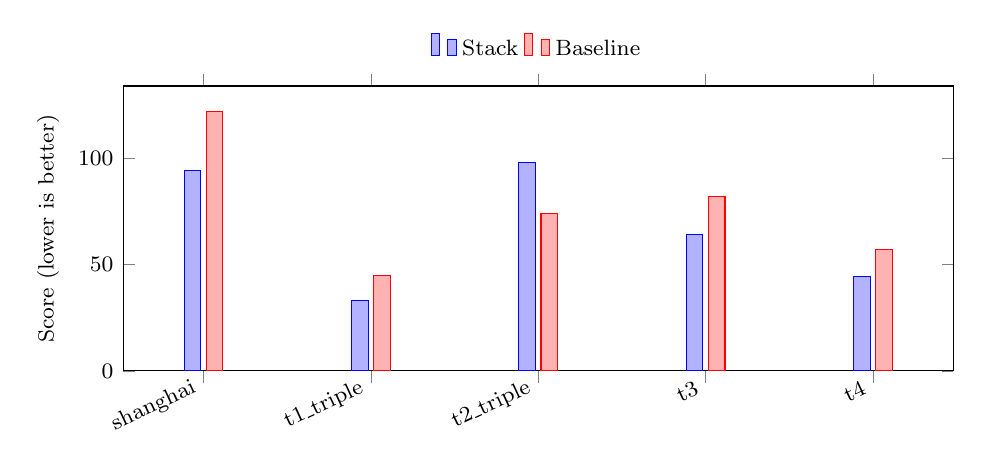
\begin{tikzpicture}
\begin{axis}[
    width=\columnwidth,
    height=5.2cm,
    ybar,
    bar width=6pt,
    ymin=0,
    ylabel={Score (lower is better)},
    symbolic x coords={shanghai,t1\_triple,t2\_triple,t3,t4},
    xtick=data,
    x tick label style={font=\footnotesize, rotate=25, anchor=east},
    ylabel style={font=\footnotesize},
    yticklabel style={font=\footnotesize},
    legend style={font=\footnotesize, at={(0.5,1.05)}, anchor=south,
                  legend columns=2, draw=none},
    enlarge x limits=0.12,
]
\addplot coordinates {(shanghai,94.5) (t1\_triple,33.05) (t2\_triple,98.25) (t3,64.2) (t4,44.45)};
\addplot coordinates {(shanghai,122) (t1\_triple,45) (t2\_triple,74) (t3,82) (t4,57)};
\legend{Stack, Baseline}
\end{axis}
\end{tikzpicture}
\caption{Stack vs.\ baseline score per track. Shorter bars are better; the stack
wins on every track except \texttt{t2\_triple}.}
\label{fig:scores}
\end{figure}

\subsection{Collision analysis}

The per-track collision logs explain most of the score variation and are
summarized in Fig.~\ref{fig:collisions}. On the four tracks run without dense
dynamic traffic (\texttt{t1\_triple}, \texttt{t2\_triple}, \texttt{t3},
\texttt{t4}), collisions are few---between one and four per run---and every one
is with \texttt{static.terrain}, i.e.\ running off the drivable surface at a
corner or boundary rather than striking another agent. The \texttt{t2\_triple}
regression corresponds directly to four such terrain collisions during that run,
consistent with a tracking or planning failure localized to that track rather
than a systemic issue: the stack scores well below baseline on the sibling
\texttt{t1\_triple} track, so the corridor geometry specific to
\texttt{t2\_triple} is the more likely culprit.

The \texttt{shanghai\_intl\_circuit} run is qualitatively different: its log
records 291 collisions, of which 220 are with static terrain and 71 are with
dynamic actors (predominantly \texttt{vehicle.tesla.model3} and
\texttt{vehicle.audi.a2}, plus a single pedestrian). This is the one track whose
log clearly reflects injected traffic, and it underscores the caveat from the
experimental setup: the Shanghai numbers were almost certainly gathered under a
different scenario configuration than the sparser tracks, so its comparison to
the baseline carries the most uncertainty despite the favorable score.

\begin{figure}[t]
\centering
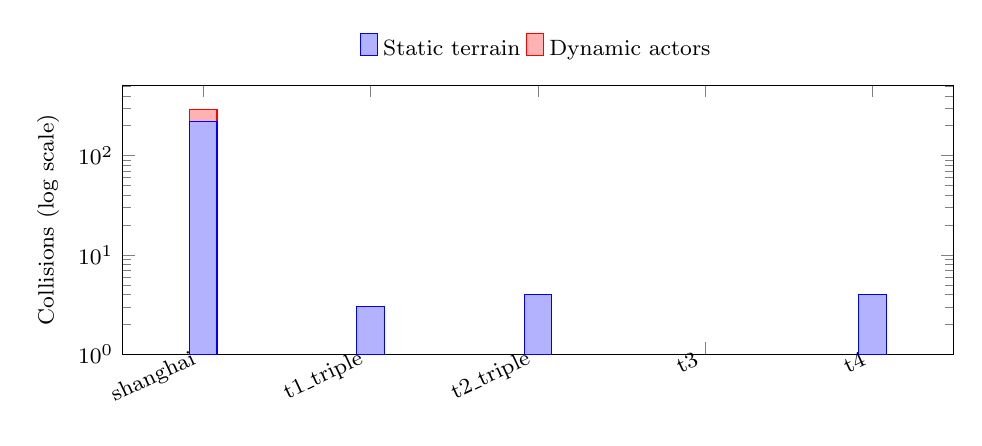
\begin{tikzpicture}
\begin{axis}[
    width=\columnwidth,
    height=5.0cm,
    ybar stacked,
    bar width=10pt,
    ymode=log,
    log origin=infty,
    ymin=1,
    ylabel={Collisions (log scale)},
    symbolic x coords={shanghai,t1\_triple,t2\_triple,t3,t4},
    xtick=data,
    x tick label style={font=\footnotesize, rotate=25, anchor=east},
    ylabel style={font=\footnotesize},
    yticklabel style={font=\footnotesize},
    legend style={font=\footnotesize, at={(0.5,1.05)}, anchor=south,
                  legend columns=2, draw=none},
    enlarge x limits=0.12,
]
\addplot+[ybar] coordinates {(shanghai,220) (t1\_triple,3) (t2\_triple,4) (t3,1) (t4,4)};
\addplot+[ybar] coordinates {(shanghai,71) (t1\_triple,0) (t2\_triple,0) (t3,0) (t4,0)};
\legend{Static terrain, Dynamic actors}
\end{axis}
\end{tikzpicture}
\caption{Collisions per track by type (log scale). Only
\texttt{shanghai\_intl\_circuit} shows dynamic-actor collisions, indicating it
was run with injected traffic.}
\label{fig:collisions}
\end{figure}

\section{Discussion and Limitations}
\label{sec:discussion}

Several limitations frame how the results should be read.

\emph{Baseline comparability.} As noted above, we could not confirm that the
reported stack scores and the reference baseline scores were captured under
identical scenario conditions. The collision logs make this concrete: only the
Shanghai run shows dynamic-actor collisions, so at least that track differs in
configuration from the others. The comparison in Table~\ref{tab:scores} is
directional context, not a controlled A/B measurement.

\emph{The \texttt{t2\_triple} regression.} The final agent underperforms the
baseline on exactly one track, and the collision log points to run-off-track
terrain contacts rather than a systemic control failure. This is the clearest
concrete weakness in the current stack and the first candidate for further
tuning.

\emph{Effective controller order.} As described in
Section~\ref{sec:integrated}, the final agent's derivative gain operates on a
previous-error term that is re-initialized every step, so the steering law
behaves as a proportional controller in practice. This likely leaves
tracking-accuracy headroom on high-curvature corners---precisely the regime
implicated in the terrain collisions---and persisting the error state across
ticks is a low-cost next step.

\emph{External dependency for Hybrid~A*.} The Hybrid~A* planner relies on a
precompiled external C++ shared library, integrated through a ctypes struct
interface. That library itself is not implemented in this repository; only the
Python-side marshalling and integration logic are.

\emph{No unified benchmark harness.} Each planner and controller variant lives
in its own module, and there is no single script in this snapshot that runs all
variants back to back and reports a comparison table. The results here are drawn
from the final integrated agent's recorded score files, not from a full
method-by-method ablation, so the paper documents \emph{which} combination was
used and how it scored rather than an isolated contribution from each component.

\emph{Adapted framework harness.} The top-level control loop is an adaptation of
Intel's CARLA ``automatic control'' example, modified for the GRAIC competition;
the planning and control agents are the original contribution of this project.

\section{Conclusion and Future Work}

We implemented and compared a broad set of planning methods (A*, Hybrid~A*,
dynamic programming, RRT, RRT*, spline smoothing, and DWA) and control methods
(PD, Stanley, Stanley+PID, LQR, and MPC) for autonomous racing in CARLA under
the GRAIC~2023 framework, and integrated the most effective combination into a
final agent that outperforms the framework's naive baseline on four of five
evaluated tracks. A per-track collision analysis localizes the single
regression to run-off-track terrain contacts on one track rather than a
systemic fault.

Four directions follow directly from the limitations above. First, root-cause
and fix the \texttt{t2\_triple} regression, using its terrain-collision log to
target the corners where the vehicle leaves the drivable surface. Second, build
a unified benchmark script that runs every variant against every track under
identical scenario conditions, so score differences can be attributed to
specific planning and control choices rather than only to the final agent.
Third, persist the steering controller's error state across ticks to recover the
intended derivative action, and evaluate the LQR and MPC controllers---which are
implemented but not reflected in the final agent---as drop-in replacements for
the current proportional law. Fourth, pin exact CARLA and GRAIC framework
versions and add a dependency manifest for reproducibility.

\begin{table}[t]
\centering
\caption{Implementation map: component to source module.}
\label{tab:impl}
\footnotesize
\begin{tabular}{ll}
\toprule
Component & Module(s) \\
\midrule
A* / grid search        & \texttt{agent\_astar.py}, \texttt{a\_star.py} \\
Hybrid A*               & \texttt{hybrid\_astar\_wrapper.py} \\
Dynamic programming     & \texttt{dynamic\_programming\_heuristic.py} \\
RRT / RRT*              & \texttt{rrt.py}, \texttt{rrt\_star.py}, \texttt{RRTStar.py} \\
Spline reference        & \texttt{agent\_SPLINE.py}, \texttt{cubicspline.py} \\
Dynamic Window Approach & \texttt{dynamic\_window\_approach.py} \\
Stanley / Stanley+PID   & \texttt{agent\_Stanley.py}, \texttt{agent\_stanley\_PID.py} \\
LQR / MPC               & \texttt{agentLQR.py}, \texttt{agentMPC.py} \\
Integrated agent (PD)   & \texttt{agent\_FINAL.py} \\
Harness / control loop  & \texttt{automatic\_control\_GRAIC.py}, \texttt{wrapper.py} \\
\bottomrule
\end{tabular}
\end{table}

\end{document}
